% answers.tex —— 1977 年·广西卷（文科） · 参考答案与详细解析片段
% 由 tools/generate_projects.py 依来源总账自 1977/1977_数学真题_广西文_试题.md + 1977/1977_数学真题_广西文_解析正文.md + 1977/1977_数学真题_广西文_答案要点.md 生成，勿手改（改源 MD 后重跑）


\begin{gktip}
固定源是题面与解答连排的书籍材料（书页 137—140，第 5 页为解答末页）。下文逐题独立推导，并与源解答对照复算，全部最终结论与源解答一致。原卷大题「一、」至「五、」已重排为连续题号 1—5，第一大题的 5 个小题对应（1）—（5）小问。需留意的源卷细节有两处：第 1(1) 题源解答首行括号内的带分数 $2\frac14$ 分子印得很淡（低倍放大下形似 $2\frac34$），按题面数值 $3\times\frac34$ 与源解答自身第二行的数值 $-2$ 判读为 $2\frac14$；第 3 题源解答「答」句把方程印作「$3x^2-(4m-1)+m^2+\frac34=0$」，漏排 $x$，系排印之误，题面方程无误。
\end{gktip}

\begin{answer}
\gksolhead{1}{}

\textbf{题目}（30 分）：

（1） 计算 $5\frac{3}{4}-2\left[\left(\frac{1}{2}\right)^2-3\times\frac{3}{4}\right]\div\frac{2}{5}$。

（2） 分解 $x^3-5x^2+4x$ 的因式。

（3） 化简 $\dfrac{1}{\sin^2\alpha}-\operatorname{ctg}^2\alpha$。

（4） 计算 $\operatorname{ctg}135^\circ+\cos(-60^\circ)-\operatorname{tg}^260^\circ+\sin30^\circ$。

（5） 不查表求 $\lg\dfrac{3}{7}+\lg70-\lg3$ 的值。

\Needspace{4\baselineskip}
\textbf{解析}

第一大题共 5 个小题，每小题 6 分。

\gksubpart{（1）}

\Needspace{5\baselineskip}
依次计算：$\left(\frac12\right)^2=\frac14$，$3\times\frac34=\frac94$，于是括号内为 $\frac14-\frac94=-2$。

\nopagebreak[4]
\[
5\frac34-2\left[\left(\frac12\right)^2-3\times\frac34\right]\div\frac25
=5\frac34-2\times(-2)\times\frac52
=5\frac34+10=15\frac34.
\]

\gksubpart{（2）}

\nopagebreak[4]
\[
x^3-5x^2+4x=x(x^2-5x+4)=x(x-4)(x-1).
\]

\gksubpart{（3）}

\Needspace{5\baselineskip}
在 $\sin\alpha\ne0$ 的条件下，

\nopagebreak[4]
\[
\frac{1}{\sin^2\alpha}-\operatorname{ctg}^2\alpha
=\frac{1-\cos^2\alpha}{\sin^2\alpha}
=\frac{\sin^2\alpha}{\sin^2\alpha}=1.
\]

\gksubpart{（4）}

\nopagebreak[4]
\[
\operatorname{ctg}135^\circ=-\operatorname{ctg}45^\circ=-1,
\qquad
\cos(-60^\circ)=\cos60^\circ=\frac12,
\]

\nopagebreak[4]
\[
\operatorname{tg}^260^\circ=(\sqrt3)^2=3,
\qquad
\sin30^\circ=\frac12.
\]

\Needspace{5\baselineskip}
原式

\nopagebreak[4]
\[
=-1+\frac12-3+\frac12=-3.
\]

\gksubpart{（5）}

\nopagebreak[4]
\[
\lg\frac37+\lg70-\lg3
=(\lg3-\lg7)+(\lg7+\lg10)-\lg3
=\lg10=1.
\]

\gkanswer{答案（1）：$15\frac{3}{4}$。}

\gkanswer{答案（2）：$x(x-4)(x-1)$。}

\gkanswer{答案（3）：$1$。}

\gkanswer{答案（4）：$-3$。}

\gkanswer{答案（5）：$1$。}

\end{answer}
\begin{answer}
\gksolhead{2}{}

\textbf{题目}（16 分）：

$P$ 是圆外一点，过 $P$ 作两条直线，一条交圆于 $C$、$A$ 两点，一条交圆于 $D$、$B$ 两点，求证 $PA\cdot PC=PB\cdot PD$。

\begin{gktip}
原源 PDF 第 3 页附有圆与两条割线、两条虚线弦的示意图；LaTeX 版按源图重绘。
\end{gktip}
\nopagebreak[4]
\begin{center}% 1977 年广西卷第 2 题：圆外一点 P 的两条割线 P-D-B、P-C-A 与两条虚线弦 AD、BC（按源卷第 3 页布局）
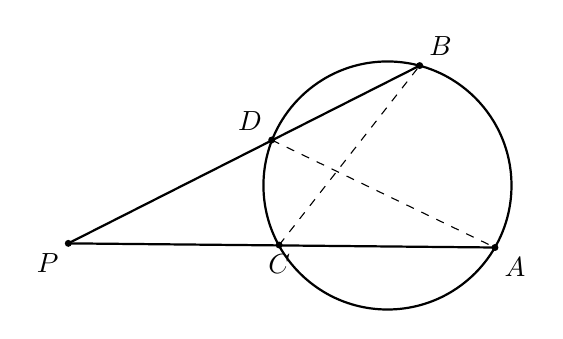
\begin{tikzpicture}[scale=1.05]
  % 圆
  \draw[thick] (0,0) circle (1.5);
  % 割线端点与圆上点（坐标手算：D、B、C、A 均在圆上，P 在圆外）
  \coordinate (P) at (-3.86,-0.70);
  \coordinate (D) at (-1.40,0.55);
  \coordinate (B) at (0.39,1.45);
  \coordinate (C) at (-1.31,-0.72);
  \coordinate (A) at (1.30,-0.75);
  % 两条割线（整段直画，保证共线）
  \draw[thick] (P) -- (B);
  \draw[thick] (P) -- (A);
  % 两条虚线弦
  \draw[dashed] (D) -- (A);
  \draw[dashed] (C) -- (B);
  % 顶点与标注
  \fill (P) circle (1.2pt) node[below left] {$P$};
  \fill (D) circle (1.2pt) node[above left] {$D$};
  \fill (B) circle (1.2pt) node[above right] {$B$};
  \fill (C) circle (1.2pt) node[below] {$C$};
  \fill (A) circle (1.2pt) node[below right] {$A$};
\end{tikzpicture}
\end{center}
\nopagebreak[4]
\Needspace{4\baselineskip}
\textbf{解析}

连接 $AD$、$BC$，构成 $\triangle PDA$ 与 $\triangle PCB$。

\Needspace{5\baselineskip}
因为 $P$、$D$、$B$ 共线，$P$、$C$、$A$ 共线，所以 $\angle PAD$ 即 $\angle CAD$，$\angle PBC$ 即 $\angle DBC$。而 $\angle CAD$ 与 $\angle DBC$ 是同弧 $CD$ 上的圆周角，故

\nopagebreak[4]
\[
\angle PAD=\angle PBC
\quad\text{（\text{同弧上的圆周角相等}）}.
\]

\Needspace{5\baselineskip}
又 $\angle P$ 是公用角，所以

\nopagebreak[4]
\[
\triangle PDA\sim\triangle PCB.
\]

\Needspace{5\baselineskip}
由相似三角形的对应边成比例，

\nopagebreak[4]
\[
\frac{PA}{PB}=\frac{PD}{PC},
\]

\Needspace{5\baselineskip}
即

\nopagebreak[4]
\[
PA\cdot PC=PB\cdot PD.
\]

\gkanswer{答案：见解析版}

\end{answer}
\begin{answer}
\gksolhead{3}{}

\textbf{题目}（17 分）：

\Needspace{5\baselineskip}
$m$ 是什么值的时候，方程

\nopagebreak[4]
\[
3x^2-(4m-1)x+m^2+\frac{3}{4}=0
\]

有相等的两个实数根。

\Needspace{4\baselineskip}
\textbf{解析}

\Needspace{5\baselineskip}
方程已含二次项系数 $3\ne0$，判别式为

\nopagebreak[4]
\[
\Delta=(4m-1)^2-4\times3\times\left(m^2+\frac34\right)
=16m^2-8m+1-12m^2-9
=4m^2-8m-8.
\]

\Needspace{5\baselineskip}
方程有相等的两个实数根 $\iff\Delta=0$，即

\nopagebreak[4]
\[
m^2-2m-2=0.
\]

\Needspace{5\baselineskip}
由求根公式，

\nopagebreak[4]
\[
m=\frac{2\pm\sqrt{(-2)^2-4\times1\times(-2)}}{2}
=\frac{2\pm2\sqrt3}{2}=1\pm\sqrt3.
\]

故 $m=1\pm\sqrt3$ 时，方程有相等的两个实数根，此时相等实根为 $x=\frac{4m-1}{6}=\frac{3\pm4\sqrt3}{6}$（与 $m$ 的取值对应）。

\gkanswer{答案：$m=1\pm\sqrt{3}$。}

\end{answer}
\begin{answer}
\gksolhead{4}{}

\textbf{题目}（15 分）：

波尔多液由胆矾、生石灰和水配制成，已知胆矾和生石灰的重量比是 $1:2$，生石灰和水的重量比是 $1:120$，问配制 $486$ 斤波尔多液需胆矾、生石灰和水各多少斤？

\Needspace{4\baselineskip}
\textbf{解析}

\Needspace{5\baselineskip}
设需胆矾 $x$ 斤，则生石灰为 $2x$ 斤；由生石灰与水的重量比 $1:120$，水为 $240x$ 斤。依题意

\nopagebreak[4]
\[
x+2x+240x=486,
\]

解得 $x=2$。所以需胆矾 $2$ 斤，生石灰 $4$ 斤，水 $480$ 斤。

验算：$2+4+480=486$；$2:4=1:2$；$4:480=1:120$，与两条已知比一致。

源卷另给连比解法：三条比化为连比 $1:2:240$，$486\div(1+2+240)=486\div243=2$（斤），即每份 $2$ 斤，得胆矾 $2$ 斤、生石灰 $4$ 斤、水 $480$ 斤，与方程法一致。

\gkanswer{答案：需胆矾 $2$ 斤，生石灰 $4$ 斤，水 $480$ 斤。}

\end{answer}
\begin{answer}
\gksolhead{5}{}

\textbf{题目}（22 分）：

已知桥的一孔为抛物线型（如图），跨度 $AB=12$ 米，桥孔高 $PO=4$ 米，建桥时每隔 $2$ 米一个撑梁，求撑梁 $C_1D_1$，$C_2D_2$，$C_3D_3$，$C_4D_4$ 各应取多长？

\begin{gktip}
原源 PDF 第 4 页附有抛物线拱桥直角坐标系示意图；LaTeX 版按源图重绘。
\end{gktip}
\nopagebreak[4]
\begin{center}% 1977 年广西卷第 5 题：抛物线拱桥 x²=−9y，顶点在原点、开口向下，
% 跨度 AB=12 米（A(−6,−4)、B(6,−4)），撑梁 C1D1…C4D4 竖直，桥面线 y=−4（按源卷第 4 页布局）
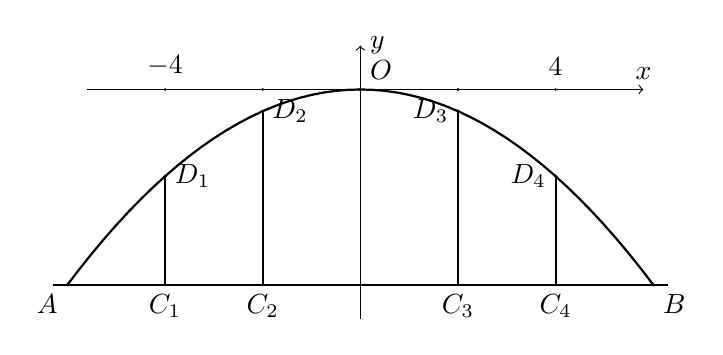
\begin{tikzpicture}[scale=0.62]
  % 坐标轴
  \draw[->] (-5.6,0) -- (5.8,0) node[above] {$x$};
  \draw[->] (0,-4.7) -- (0,0.9) node[right] {$y$};
  \fill (0,0) circle (1.1pt) node[above right] {$O$};
  % 抛物线 y = -x^2/9（顶点在原点，开口向下）
  \draw[thick, domain=-6:6, samples=49] plot (\x, {-\x*\x/9});
  % 桥面线（弦 AB 所在水平线）
  \draw[thick] (-6.3,-4) -- (6.3,-4);
  \fill (-6,-4) circle (1.1pt) node[below left] {$A$};
  \fill (6,-4) circle (1.1pt) node[below right] {$B$};
  % 四根撑梁（x=±2、±4）
  \foreach \i/\xx in {1/-4, 2/-2, 3/2, 4/4} {
    \pgfmathsetmacro{\yy}{-\xx*\xx/9}
    \draw[thick] (\xx,-4) -- (\xx,\yy);
    \fill (\xx,-4) circle (1pt) node[below] {$C_{\i}$};
    \pgfmathtruncatemacro{\side}{\xx>0 ? -1 : 1}
    \ifnum\side<0
      \fill (\xx,\yy) circle (1pt) node[left] {$D_{\i}$};
    \else
      \fill (\xx,\yy) circle (1pt) node[right] {$D_{\i}$};
    \fi
  }
  % x 轴刻度点与标注（−4 与 4）
  \foreach \xx in {-4,-2,2,4} { \fill (\xx,0) circle (0.9pt); }
  \node[above] at (-4,0.08) {$-4$};
  \node[above] at (4,0.08) {$4$};
\end{tikzpicture}
\end{center}
\nopagebreak[4]
\Needspace{4\baselineskip}
\textbf{解析}

\Needspace{5\baselineskip}
以抛物线顶点为坐标原点、对称轴为 $y$ 轴建立直角坐标系，则抛物线开口向下，设其方程为

\nopagebreak[4]
\[
x^2=-2py
\qquad\text{（$p>0$）}.
\]

\Needspace{5\baselineskip}
跨度 $AB=12$ 米，故 $B$ 点横坐标为 $6$；桥孔高 $PO=4$ 米，故 $B(6,-4)$。代入方程：

\nopagebreak[4]
\[
6^2=-2p\times(-4)
\qquad\Longrightarrow\qquad
p=\frac92,
\]

\Needspace{5\baselineskip}
所以抛物线方程为

\nopagebreak[4]
\[
x^2=-9y.
\]

\Needspace{5\baselineskip}
建桥时每隔 $2$ 米一个撑梁，两端各留 $2$ 米，故四根撑梁位于 $x=\pm2$、$x=\pm4$。由对称性只需计算右半两根：

\nopagebreak[4]
\[
D_3\left(2,-\frac49\right),
\qquad
D_4\left(4,-\frac{16}{9}\right).
\]

\Needspace{5\baselineskip}
$C_3$、$C_4$ 在桥面线 $y=-4$ 上，故

\nopagebreak[4]
\[
|C_3D_3|=4-\frac49=\frac{32}{9}=3\frac59\ \text{（\text{米}）},
\]

\nopagebreak[4]
\[
|C_4D_4|=4-\frac{16}{9}=\frac{20}{9}=2\frac29\ \text{（\text{米}）}.
\]

\Needspace{5\baselineskip}
由抛物线的对称性，

\nopagebreak[4]
\[
|C_1D_1|=|C_4D_4|=2\frac29\ \text{（\text{米}）},
\qquad
|C_2D_2|=|C_3D_3|=3\frac59\ \text{（\text{米}）}.
\]

与源解答一致。

\gkanswer{答案：撑梁 $C_1D_1$、$C_4D_4$ 长为 $2\frac{2}{9}$ 米，$C_2D_2$、$C_3D_3$ 长为 $3\frac{5}{9}$ 米。}

\end{answer}